\subsection{Generated Worlds}

In this section are shown the three different Generated Worlds, one for each component analyzed through Alloy.\\

\lstinputlisting[language=alloy]{./Chapters/Chapter4/AlloySourceCode/Predicates.als}

\begin{figure}[H]
  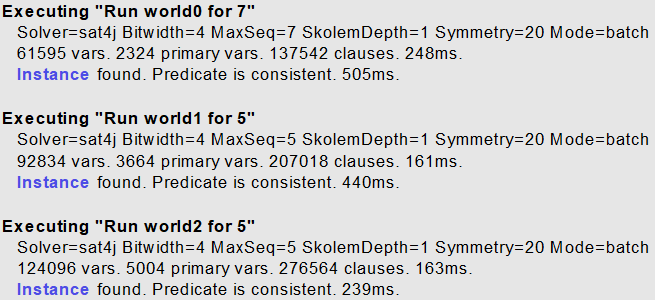
\includegraphics[width=\textwidth,height=\textheight,keepaspectratio]{./Images/Alloy/predicatesExecution.png}
  \caption{Alloy Analysis Results}
\end{figure}

\begin{center}
\begin{figure}[H]
\centering
  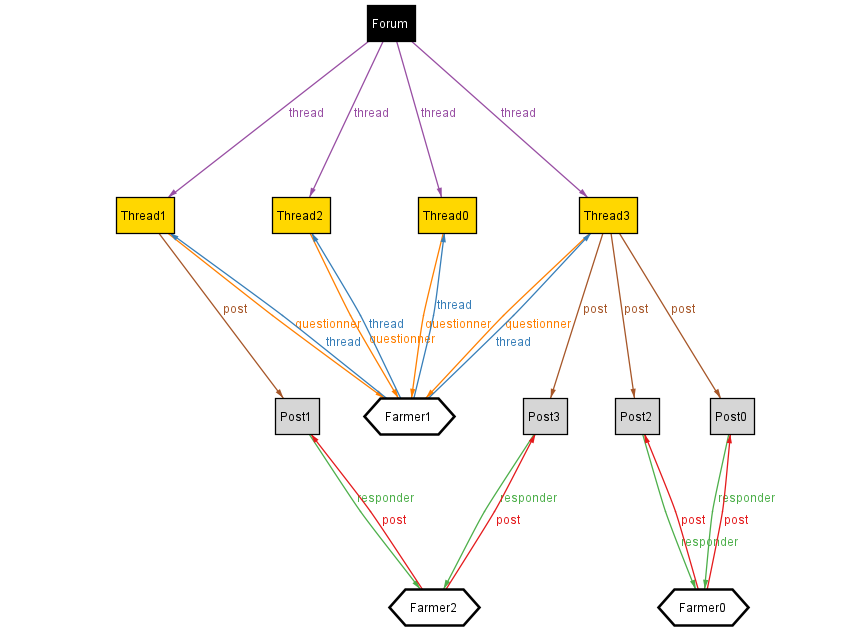
\includegraphics[angle = 90,scale= 0.55]{./Images/Alloy/DiscussionForum.png}
    \caption{Generated World0 - Discussion Forum}
    \label{fig:LandscapeFigure}
\end{figure}
\end{center}

\begin{center}
\begin{figure}[H]
\centering
  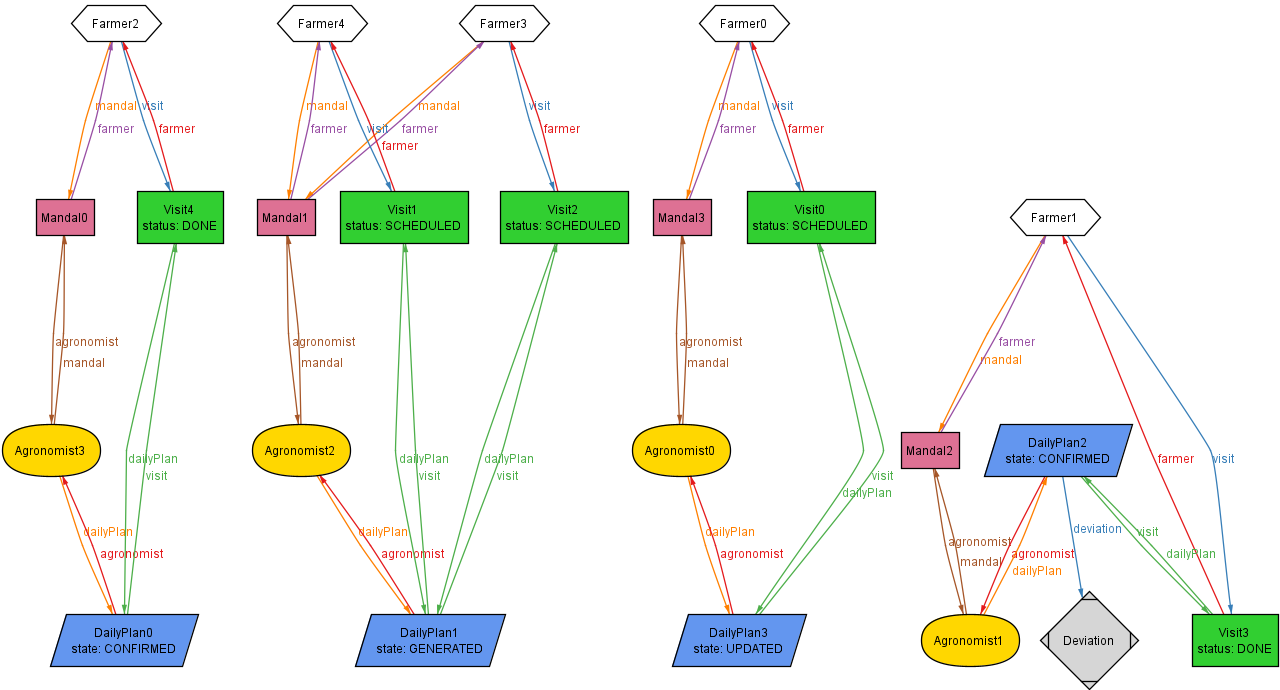
\includegraphics[angle = 90,scale= 0.4]{./Images/Alloy/DailyPlan.png}
  \caption{Generated World1 - Daily Plan}
    \label{fig:LandscapeFigure}
\end{figure}
\end{center}

\begin{center}
\begin{figure}[H]
\centering
  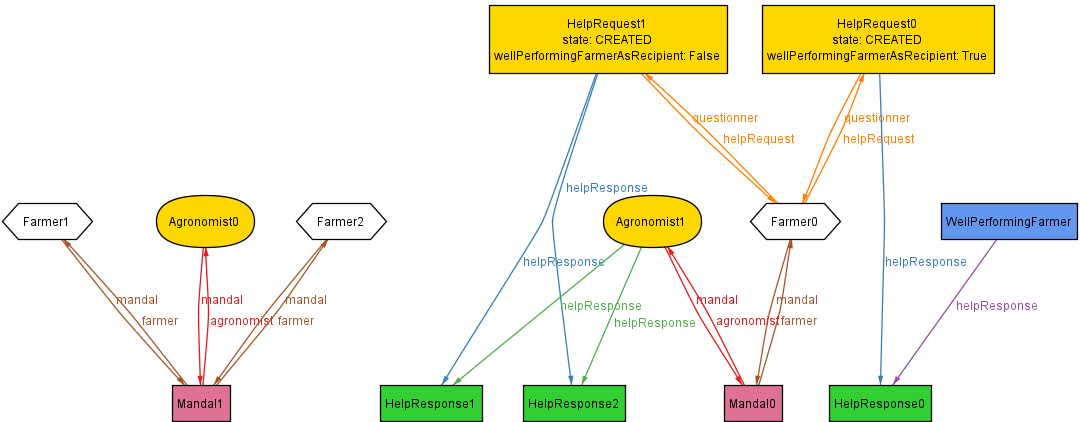
\includegraphics[angle=90,scale= 0.5]{./Images/Alloy/HelpRequest.png}
  \caption{Generated World2 - Help Request}
    \label{fig:LandscapeFigure}
\end{figure}
\end{center}
